\documentclass[a4paper,10pt]{article}
\usepackage{graphicx}
\usepackage{verbatim}
\usepackage{subfig}
\usepackage{float}
\usepackage[spanish]{babel}   %ver bien como es
\usepackage[utf8]{inputenc}

\begin{document}

\tableofcontents

\newpage


\section*{Introducci\'on}
\addcontentsline{toc}{section}{Introducci\'on}

El objetivo de este trabajo es brindar posibles soluciones para el desarrollo de un software, el mismo ser\'a utilizado en una cadena de pizzer\'ias llamada "Pizza Hack". El análisis del software a desarrollarse fue solicitado por la cadena, que además puntualizó determinados objetivos que de antemano consideran importantes.


En conjunto con las explicaciones en lenguaje natural se incluyen modelos de objetivos y de agentes. Estos modelos permiten plasmar sintéticamente, de manera gráfica, una idea general de las características que identificamos en el conjunto de las posibles soluciones y que a su vez describen el problema. 

Una de las ventajas de los modelos de objetivos es que permiten identificar las relaciones entre los distintos objetivos de alto nivel, como así también descomponerlos en objetivos más concretos. Ésta descomposición permite a su vez delegar la responsabilidad del cumplimiento de un objetivo en una entidad activa, que se denomina agente, permitiendo de esta manera desarrollar soluciones alternativas con diferente grado de intervención del software en sí. Las alternativas que se generen a partir de la exploración de las posibles soluciones también se podrán ver representadas en forma esquemática. 

En los diagramas de contexto se podrán explorar con más detalle las interacciones que se darían en algunas de las variantes de nuestras posibles soluciones y entender mejor el rol que cumple cada agente.

De acuerdo a los objetivos priorizados por la cadena, el sistema debe tener las siguientes características:


El sistema pedido debe ser un sistema distribuido, es decir, debe operar en cada local por separado. Para realizar este an\'alisis para el posterior desarrollo del sofware se debi\'o pensar en que dicha cadena pretende ofrecer a sus clientes un men\'u en com\'un en todos los locales, es decir, mismo plato y mismo precio. Dicho men\'u debe poder ser modificado, por ejemplo si se desea cambiar alg\'un precio y agregar o quitar alguna variedad de pizza. Por otro lado, el sistema a desarrollar debe poder tener un manejo del nivel de stock, para que se pueda saber cuando se tienen que reponer los ingredientes. Adem\'as, conocer la cantidad de los elementos necesarios para realizar cada variedad que hay al momento, permite saber si un pedido va a poder ser realizado o no, de esta forma se garantiza que no se cancelen pedidos por falta de ingredientes. En el caso de que el cliente quiera pedir una variedad de pizza que no se pueda realizar en el local donde la est\'a pidiendo, se tiene que poder saber si en alg\'un otro local de la cadena hay stock como para realizar dicho pedido y contar con la posibilidad de reservar los ingredientes, al menos hasta que el cliente la retire en el otro local en cuestion. En el caso de que el cliente no pase a retirar el pedido se tiene que poder recuperar los ingredientes reservados. Finalmente, este informe brinda el an\'alisis de dicho software y requerimientos del hardware para el sistema.



Cosas que dijo la catedra:

acá debería figurar todo lo necesario como para que un
lector no iniciado en el tema entienda el propósito general del
sistema que van a describir. Puede citar algunos fragmentos del
enunciado si lo consideran necesario, pero NO DEBE SER una copia del
enunciado.

\newpage
\section*{Presunciones}
\addcontentsline{toc}{section}{Presunciones}

Cosas que dijo la catedra:

acá deberían listar aquellas cuestiones que asumieron
por encima del enunciado. Estas cuestiones pueden provenir de alguna
consulta con docentes. También pueden provenir de alguna especulación
o interpretación que el grupo hizo.
\noindent
\textbf{Tiempo de pedido:} asumimos que dos clientes no puede hacer un pedido de forma simultánea. Esta presunción permite simplificar el cumplimiento del objetivo relacionado a no dejar que se pueda cancelar un pedido a un cliente luego de que fue hecho, dado que establece un claro orden entre ellos. \\
\textbf{Tiempo de pedido a distancia:} asumimos que, ante un pedido a `distancia' (es decir, de un local a otro), un cliente pierde el interés en buscar dicho pedido luego de un \textit{time out} pautado de antemano. Esta presunción nos ayuda a poder cumplir, por un lado, el objetivo relacionado a permitir dicha compra `a distancia' y, por otro, a poder mejorar el manejo de stock al cancelar el pedido luego de pasado el \textit{time out}, y de esta forma recuperar el stock reservado para éste. Esto se logra sin violar los objetivos relacionados al funcionamiento de las ventas (no cancelar pedidos hechos), dado que se interpreta como que el cliente es el que cancela el pedido al no presentarse y no el local.\\
\textbf{No hay actualizaciones simultáneas:} Habiéndose hecho especial énfasis en que la solución informática no debe ser centralizada, en caso de haber actualizaciones simultáneas se debería arbitrar, de manera distribuída, cuál de las actualizaciones es la que corresponde propagar a la totalidad de las sucursales. Siendo ésta una situación que no consideramos muy común, parece razonable suponer que no hay actualizaciones simultáneas de las variedades del menú. De ésta manera dicho arbitraje no es necesario. \\ 
\newpage
\section*{Vistas}
\addcontentsline{toc}{section}{Vistas}

Cosas que dijo la catedra:

está sería la parte principal del TP. Acá irían los
diagramas y los escenarios representativos de uso. No necesariamente
tiene que ser una gran sección, sino que pueden partirla por
funcionalidades y a su vez por tipo de vista o de la forma que crean
más pertinente. Esta sección NO DEBE SER una simple seguidilla de
figuras sueltas. Debe estar acompañada de tantas explicaciones como
sean necesarias para que se aprecie un hilo conductor.

\section*{Diagrama de contexto}
El siguiente diagrama de contexto muestra los agentes involucrados en interacciones con una solución que se orienta a la automatización. 

\paragraph{Proveedor:}
El proveedor es el encargado de reponer el stock a pedido de nuestro local. Incluye todo el sistema de compra y transporte de productos hasta el local.
\\
\paragraph{Menú Electrónico:}
El menú electrónico consiste en un menú interactivo ofrecido a los usuarios a través de iPADs, los cuales son asignados de a uno por mesa. En éste pueden distinguirse las distintas variedades de productos (no únicamente pizzas, sino también bebidas y postres) y sus correspondientes precios. A su vez, en distintos colores se puede distinguir si el producto está o no disponible (es decir, si hay stock de ingredientes para preparalo) y si, en caso de que no haya, puede o no ser pedido en otro local en que sí haya stock, ofreciéndo al cliente la opción de elegir en qué local puede hacer el pedido.
\\
\paragraph{Cliente:}
El cliente que entra al local. Se refiere tanto a individuos como a grupos.
\\
\paragraph{Personal:}
Se refiere al conjunto de personas que trabajan en el local, éstos son: los mozos, el cajero y los cocineros.
\\

La solución presentada en general prioriza la satisfacción del cliente, ya que al ocuparse el software de manera casi íntegra del manejo de stock, resulta posible descontar inmediatamente la disponibilidad de un determinado ingrediente al registrarse un pedido, incluso antes de iniciarse su preparación. Esto evita que al ocurrir varios pedidos concurrentes se acepten pedidos para los cuáles no se dispone de stock suficiente.

Por otra parte, aún cuando el personal no hubiera registrado la escacez de un ingrediente, el sistema lo informaría logrando la reposición del mismo. Debido a posibles imprecisiones en las cantidades de ingredientes registradas para cada receta es necesario que el personal periódicamente haga un inventario completo de las existencias y actualice las cantidades disponibles mediante una interfaz gráfica que será provista por el software.

Es importante destacar que en este caso estamos considerando la comunicación entre sucursales parte del sistema a desarrollarse. En este sentido este sistema no es completamente tolerante a fallas, ya que en el caso de falla por parte del proveedor de servicio de Internet, el sistema se vería inhabilitado para realizar operaciones entre sucursales. Se podría agregar un modo de funcionamiento manual, pero no garantizaría los beneficios del sistema automatizado y además agregaría costo en concepto de funcionalidades que sólo se utilizarían en caso de falla total del servicio de Internet. 

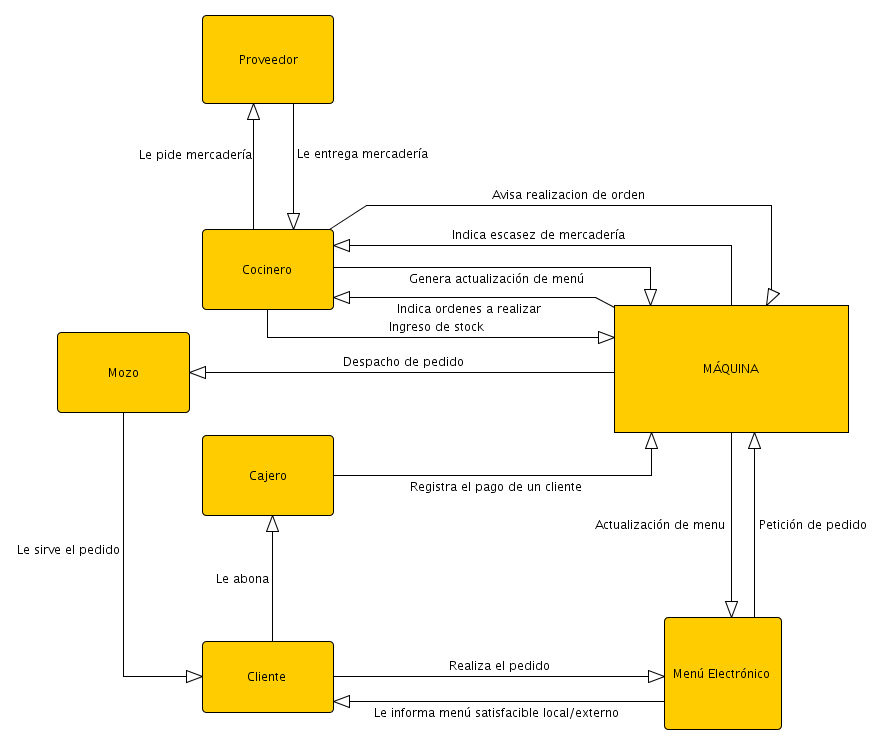
\includegraphics[width=400pt]{imagenes/agentes_automatico.png}



\section*{Modelo de objetivos}
\addcontentsline{toc}{subsection}{Modelo de objetivos}
\subsection*{Objetivos}
\addcontentsline{toc}{subsubsection}{Objetivos}
\noindent

El siguiente diagrama expresa algunos de los objetivos requeridos por la cadena y que consideramos troncales.


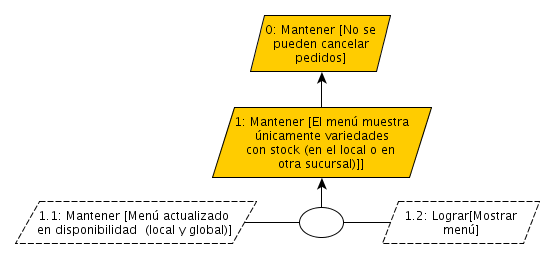
\includegraphics[width=400pt]{imagenes/objetivos_principales.png}

Los objetivos planteados garantizan que un pedido no será cancelado una vez confirmado. Es decir, un pedido no será cancelado por falta de ingredientes para prepararlo. 

Para lograr esto proponemos que el menú sólo muestre variedades de pizza disponibles, ya sea en la sucursal en la que se está consultando el menú, o eventualmente en otra sucursal, obviamente indicando dicha particularidad.

El objetivo de mantener el menú actualizado en cuanto a disponibilidad plantea a su vez varios objetivos relacionados, por lo que a continuación nos extendemos en su descripción.

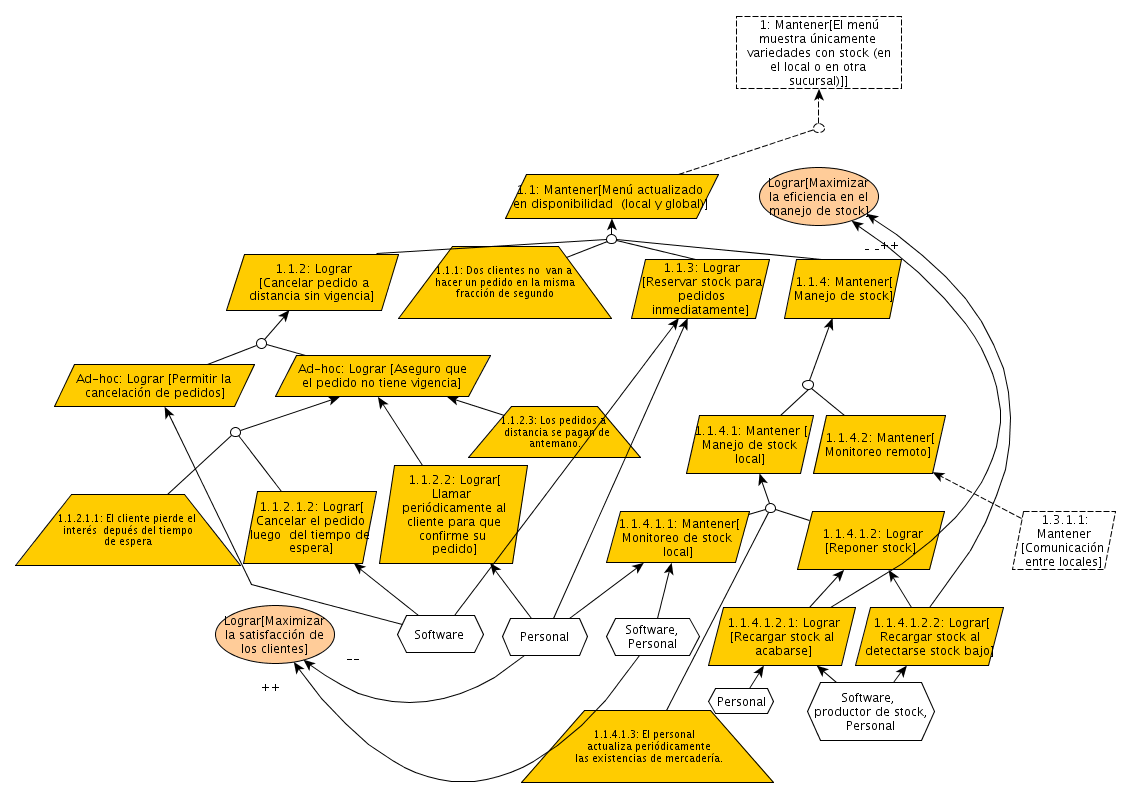
\includegraphics[width=400pt]{imagenes/objetivos_menu.png}

Como se puede apreciar, surge una gran cantidad de objetivos en algún sentido más simples, algunos de los cuáles consideramos que pueden ser concretados por un agente en particular. En estas asignaciones de objetivos van a surgir las diferentes variantes de la solución propuesta. 

En el anterior diagrama se muestra una dependencia entre el objetivo 1.1 y el 1.1.4. Estrictamente parecería que lo único que es relevante al objetivo 1.1 con respecto al manejo de stock es el monitoreo, tanto local, o restringido a la sucursal en la que se usa el menú, como global, o remoto, del mismo. Por cómo pensamos la solución de software, esta dependencia en realidad existiría, ya que el manejo de stock estaría intimamente ligado a la exactitud y actualidad de los datos obtenidos mediante el monitoreo. Es por eso que mantenemos esa jerarquía.


A continuación nos enfocaremos en el objetivo 1.1.4.1.1. 
\subsubsection*{Mantener [Monitoreo de stock]}
Como vemos, consideramos que existe la opción de asignar la concreción de este objetivo por un lado al Personal, y por otro al Software en conjunto con el Personal. Esta apreciación merece algunas observaciones.
En primer lugar, asignarlo al Personal consistiría en que los cocineros actualicen con cada pedido el stock disponible, descontando manualmente, mediante una interfaz provista por el software, los ingredientes utilizados en cada caso.  


La opción de asignarlo al Software en conjunto con el Personal consiste en que el software asocie cada variedad de pizza a los ingredientes, con sus cantidades correspondientes, necesarios para prepararla. De esta manera, en el instante mismo en que se genera un pedido, el sistema actualizaría las cantidades disponibles de cada ingrediente de manera automática y sin intervención del personal. Sin embargo, por no ser exactas las cantidades registradas en la receta, sería necesario que el Personal haga un inventario completo periódicamente y actualice la disponibilidad de ingredientes con los valores reales.

En este sentido, la expectativa 1.1.4.1.3 tiene varias implicaciones. En el caso de cumplir el objetivo 1.1.4.1.1 con una solución mixta, el Personal debería actualizar las existencias con una periodicidad dada por la eventual inexactitud de las recetas. En el caso de cumplirlo sólo mediante la participación del Personal, sería necesario que la actualización de las existencias fuera casi permanente.

La decisión respecto del objetivo 1.1.4.1.2 está relacionada con las consideraciones mencionadas, ya que, en caso de tenerlo, sería deseable aprovechar las capacidades de monitoreo de stock provistas por el software para alertar al personal de manera que realice un pedido al proveedor si fuera necesario. Las dos políticas de recarga de stock son mencionadas debido a que, si bien la recarga de stock al acabarse es mejor en relación a maximizar la eficiencia en el manejo de stock, es claramente deficiente en relación a la satisfacción del cliente, ya que permite que haya variedades de pizza no disponibles.


La realización de pedidos a distancia, reservando el stock necesario para prepararlo, está relacionada con la precisión del monitoreo de stock. Por lo que ahora nos centraremos en el objetivo 1.1.2:
\subsubsection*{Lograr [Cancelar pedido a distancia sin vigencia]}
Como mencionamos, al realizar un pedido a distancia, los ingredientes para realizar dicho pedido deben ser reservados, garantizando de esa manera que, al llegar el cliente a la sucursal, su pedido todavía puede realizarse. El conflicto surge si un cliente pierde el interés en su pedido y no lo va a retirar.
Este objetivo trae aparejados varios obstáculos, ya que en principio se desearía evitar cancelar un pedido excepto en casos en los que se pudiera asegurar que el cliente perdió el interés en su pedido, pero por otra parte, no es deseable que se mantengan reservados ingredientes que no van a ser utilizados.
Las opciones que a continuación detallamos tienen cada una sus propias ventajas y desventajas, por lo que eventualmente sería necesario que un experto de dominio aporte más información.


Una forma de resolver este conflicto es asumir que los clientes nunca van a retirar su pedido pasado cierto tiempo, debido a que pierden el interés. Siguiendo este razonamiento es seguro volver a disponer de los ingredientes reservados. La limitación de este enfoque es la falta de flexibilidad, ya que un cliente podría retrasarse mucho más de lo común y aún así pasar a buscar su pedido luego de un tiempo considerable.

Una sofisticación de esta idea es requerir información de contacto al realizar un pedido a distancia, un teléfono celular por ejemplo. Y periódicamente llamar al cliente para confirmar que mantiene su interés, dando de baja el pedido en caso contrario. Esta opción, mucho más flexible que la anterior, requiere la participación del Personal y por otra parte requiere que los clientes provean algún tipo de medio de contacto para tener alguna utilidad.

Por último, si los clientes pagaran su pedido en la sucursal en la que se encuentran, aún si el mismo se entregara en otra, sería razonable suponer que lo va a pasar a buscar, por lo que no habría pedidos a distancia que perdieran la vigencia y no sería necesario cancelarlos.

Más adelante retomaremos el objetivo 1.3.1.1, referido a la comunicación entre locales.
El resto de los objetivos tienen nombres lo suficientemente explicativos, por lo que vamos a retomar los objetivos planteados por la cadena.



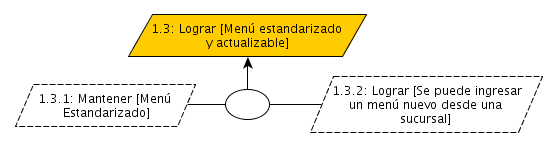
\includegraphics[width=400pt]{imagenes/objetivos_menu_estandarizado.png}

Entre las pautas se menciona la necesidad de poder actualizar el menú y la restricción de que el menú sea el mismo para todas las sucursales. A continuación nos enfocamos en cómo mantener un menú estandarizado.



\textbf{Mantener[Menú estandarizado]:} para mantener un menú estandarizado simplemente tenemos que aseguranos que sea el mismo en todos los locales, sean cual sean las actualizaciones que se han realizado (de variedades, precios, etc). Para ello únicamente tenemos que asegurar que se mantenga la comunicación entre los locales. \\
\textbf{Lograr[Se puede ingresar un menú desde una sucursal]:} para lograr un menú actualizable tenemos que asegurarnos de que se puedan realizar las actualizaciones pertinentes de éste. \\
\textbf{Lograr [Autorizar el ingreso de un menú nuevo desde una sucursal]:} pensamos varias formas de manejar esto: una de ellas consiste en que los locales pueden realizar actualizaciones en un momento determinado del día, bien puede ser esto a una hora prefijada de antemano o bien puede ser cuando cierra el local a la noche. Si el local no respeta estos horarios no le es permitido ingresar la actualización. Otro caso a considerar es cuando se cae la conexión del sistema, en caso de usar comunicación automatizada, en cuyo caso tampoco se permiten las actualizaciones, dado que sería una actualización local y el menú debe ser el mismo en todos los lugares. Por otra parte se debe verificar de alguna manera que quien intenta ingresar un nuevo menú esté autorizado. Puede utilizarse una contraseña o crear cuentas para los distintos usuarios del sistema. \\
\textbf{Lograr [Recargar stock al detectarse el nivel de stock]:} para esto planteamos dos alternativas. La primera es recargar el stock cuando se agote completamente, que es más eficiente en el manejo de stock porque involucra que se carga sólo las veces necesarias (recordar que cada carga tene su costo, por ejemplo el pago de transporte al proveedor). La segunda es recargar el stock cuando se detecte bajo stock, esto no es eficiente en términos de manejo de stock, pero ayudaría enormemente a mantener un menú rico en disponibilidad de productos, lo cual conllevaría a perder menos clientes debido a que sus pedidos no pudieron ser satisfechos.\\
\textbf{Lograr [Cancelar pedido a distancia]:} para cumplir este objetivo planteamos dos alternativas: por un lado el local es el que cancela el pedido al excederse un cierto \textit{time out}, mientras que por el otro el local llama periódicamente al cliente para confirmar que éste mantiene su interés. La primera se apoya en una presunción del dominio que indica que un cliente pierde el interés en realizar la compra luego de pasado cierto tiempo, en cuyo caso se cancela el pedido de forma automática. El segundo caso, en cambio, ofrece una mayor flexibilidad al cliente, que puede demorar más tiempo en llegar a la sucursal correspondiente. Pensamos que esta última opción de alguna forma mejora la satisfacción del cliente al permitirle mayor flexibilidad en el manejo de su tiempo.\\
\textbf{1.1.4.1.2.1 Lograr [Recargar stock al acabarse]:} mediante el agente controlador de stock se da aviso de la falta de stock. Los agentes pueden ser: una persona o un controlador de stock informatizado. El controlador de stock informatico (implementado en disitintas tipos de tecnologia) se comunica (mediante distipos tipos de comunicacion)con distintos proveedores.La persona llama al proveedor.\\
\textbf{1.1.4.1.2.2 Lograr [Recargar stock al detectarse stock bajo]:} idem anterior\\
\textbf{1.1.4.1.2 Lograr[Reponer stock]:}para cumplir este objetivo es necesaria una politica de reposicion.\\
\textbf{1.1.4.1.1 Mantener [monitoreo stock local]:} Se quiere lograr tener un control preciso de la disponibilidad de ingredietes. La estrategia a utilizar es la de descontar con cada orden los ingredientes utilizados dicha tarea se puede asignar a dos agentes diferentes. Por un lado esta tarea se puede asignar al personal del local para realizar el monitoreo de manera manual. Por otro lado, dicho objetivo puedo encontrarse a cargo de un controlador de stock informatizado en cada local que periodicamente se contrasta con un inventario total.\\
\textbf{1.1,4,1 Mantener [manejo de stock local]:} Se mantiene un monitoreo de la disponibilidad de ingredientes y se los repone cuando sea necesario.\\
\textbf{1.1.4.2 Mantener [monitoreo remoto]:} Se debera conocer el stock de las otras sucursales. \\
\textbf{1.1.4 mantener [manejo de stock] :} se debera conocerla disponibilidad de ingredientes tanto de la sucursal local como de las otras.y se debera mantener el stock en niveles aceptables.\\
\textbf{1.1.3 Lograr [reservar stock opara pedidos inmediatamente]:} Se debera reflejar la disminucion de la disponibilidad de ingredientes al momento de la produccion del pedido. \\
\textbf{1.1.2 Lograr [cancelar pedido a distancia]:} Se permitira cancelar el pedido a distancia en los casos que el cliente pierda el interes.\\
\textbf{1.1.2.2 Lograr [llamar periodicamente al cliente para que confirme su pedido]:}.Se contactara al cliente telefonicamente para uqe confirme que mantiene su interes por el pedido. este objetivo puede ser asignado al personal que debera ademas ocuparse de obtener la informacion de contacto.\\
\textbf{2.1.1 El Cliente pierde el interes despues del tiempo de espera:} Hipotesis de de dominio luego de un determinado tiempo se asume que el cliente no va a retirar el pedido.\\
\textbf{1.1.2.1.2 Lograr cancelar el pedido despues de un tiempo de espera:} Luego de expirar el tiempo de time out el controlador de stock envia una senal indicandole al local una actualizacion de stock.\\
\textbf{1.3.1.1.2 Sistema de sincornizacion de datos:}  mediante el sistema informatico de internet se mantiene la comunicacion automatica entre diferentes locales en su forma optima(en contraposicion al otro agente).\\

%Se debera permitir aceptar pedidos de una sucursal remota y a la vez poder realizar los pedidos que no sean satisfechos pro el local en cuestion a otra sucursal de la cadena que si disponga del stock necesario para cubrir el pedido del cliente.

\newpage
\section*{Escenarios}

El dia 29/02/2004 a las 12:47:59 entran simultaneamente al local de pizza Hack (sucursal barrio mitre) Alan Faina, Sergio Mazza, Tomas Anchorena y 4taPersona en busqueda de una buena sapi. Alan se sienta en la mesa nro 1, tomas en la mesa nro 2, sergio mazza en la 3 y la 4ta en la mesa 4. 
\begin{itemize}\item
\item pedir en otra sucursal e ir
\item peidr en otra y no ir
\item pedir y que no haya
\item pedir y que haya y que el siguiente no tenga
\item que se quede sin stock y pedir stock.
\end{itemize}

\newpage
\section*{Discusi\'on}
\addcontentsline{toc}{section}{Discusi\'on}

Cosas que dijo la catedra:

debe contener un análisis general de las distintas
alternativas y su impacto en los objetivos blandos. NO DEBE SER una
lista de lo que ya se puede desprender del diagrama. Debe ser un
análisis más cualitativo y "a vuelo de pájaro" que permita entender
este asunto en pocas palabras. Esta sección también es ideal para que
vuelquen las cosas que puedan haberles quedado "flojas" o no cerradas
del todo: por ejemplo los potenciales conflictos entre objetivos, los
aspectos que podrían hacer que todo el sistema no funcione como
desean, etc.

\newpage
\section*{Conclusiones}
\addcontentsline{toc}{section}{Conclusiones}

Cosas que dijo la catedra:

mencionar brevemente de qué formas les resultó más
sencillo encarar el TP. Por ejemplo en qué orden realizaron los
diagramas, qué aspectos presentaron las mayores dificultades, etc.




\end{document}
